\chapter{绪论}
\section{研究背景}
近年来,由于云计算灵活、便捷、可扩展的特性,越来越多电子商务、社交网络、金融、医药等领域的企业都选择将其服务应用部署于云计算环境中。在云计算环境中,这些服务应用会被部署在复杂庞大、跨协议的分布式集群上。随着分布式集群中的软硬件变迁、技术升级、配置更新等,各种故障时有发生,如资源争用死锁、软件运行错误、硬件故障等。另外,分布式集群结构的复杂性和资源的共享关联性会形成阻力,导致运维人员很难快速准确地发掘、分析分布式集群故障数据,进而导致故障未被及时发现并进一步扩散,最终导致应用不可用,造成巨大的经济损失。例如,云提供商AmazonWeb Service(AWS)在2015年9月20日上午2:13到7:10之间发生了一次服务宕机,当时用户无法访问Netflix,Tinder,Airbnb,Reddit和IMDb等流行的在线服务,失败的根源在于美国东部地区亚马逊DynamoDB服务的读写操作异常。

因此,如何借助人工智能技术辅助运维人员自动检测、分析、预测故障成为了研究的热点及难点。近些年被提出的AIOps就尝试将人工智能技术与运维相结合,通过机器学习的方法来提升运维效率。但大量已有AIOps方案均使用历史数据训练感知机、贝叶斯、随机森林等机器学习模型,用于异常检测、异常分类、故障预测以辅助运维,都停留在算法层面,缺乏对知识的沉淀、表示和推理。分布式集群中可用的信息是庞大且多样的,有组件间的拓扑关系、硬件的指标时序数据、软件的运行日志数据,如图\ref{cloud-environment}所示为分布式集群的示意图。组件间的拓扑关系指明了组件间的交互、依赖等关系,如slb会调控多台ecs实现负载均衡;硬件的指标时序数据记录了硬件的内存占用率、读写速度、cpu负载率等随时间的变化曲;软件的运行日志数据记录了各个微服务在具体时间戳打印的日志内容。分布式集群中的这些信息不仅能用来训练模型以解决某个检测、分类或预测的子任务,还可以将历史数据中隐含的运维知识沉淀为结构化的知识图谱。生成的知识图谱对于云服务提供商,可以为客户提供更稳定的服务以增加收益。对于运维人员,可以更直观,更有效地管理分布式集群减少人力消耗,并做出可解释、可靠的运维决策。对于云应用程序开发人员,可以减少应用程序部署,迭代和发布的阻力。
\begin{figure}[htbp]
    \centering
    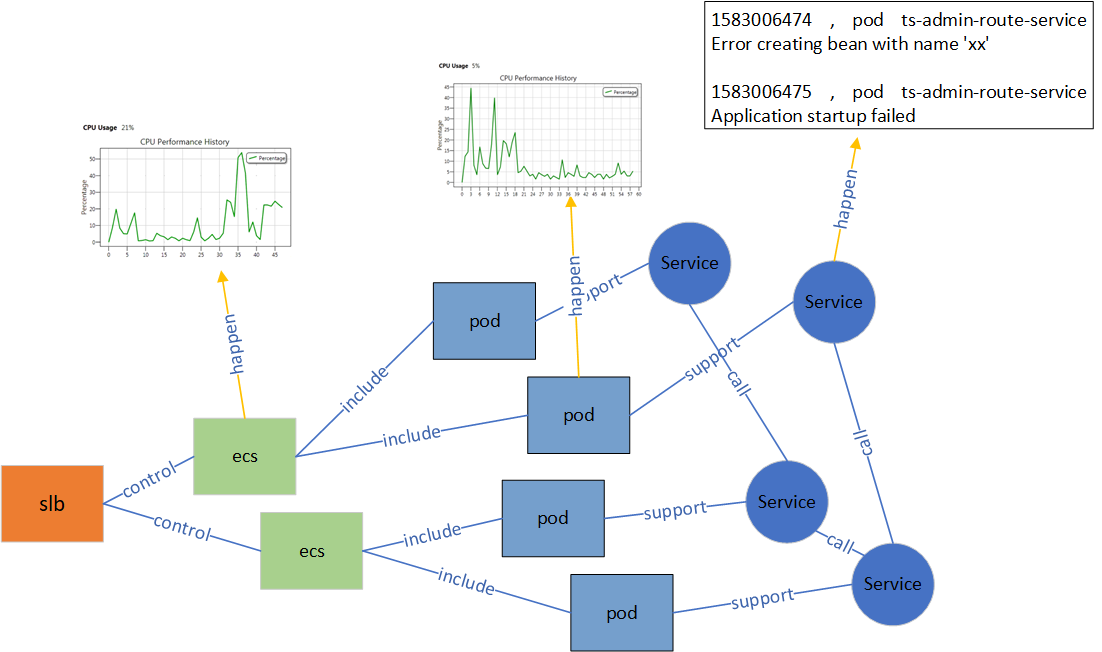
\includegraphics[width=.6\textwidth]{cloud-environment.png}
    \caption{集群schema示意图\label{cloud-environment}}
\end{figure}

首先,本文分析了现有的云计算场景知识图谱构建方案,发现这些方案仅使用了分布式集群部分信息且挖掘的数据特征有限,导致所构建的图谱比较片面且质量不佳。本文扩展了数据特征,且收集横跨软硬件的信息构建了组件-事件知识图谱。其次,本文针对云计算下异常沿组件图传播、前文事件序列触发后续事件的特性,提出了多层注意力机制的知识图谱表示学习方案。最后,本文将多层注意力机制的知识图谱表示学习模型所学习到的事件嵌入表示引入实时事件序列的故障预测,从而将运维知识引入到故障预测中,增强了预测结果的可靠性。

\section{研究现状}
针对分布式集群信息多样繁杂不易整合、运维知识表示不足、故障难以预知等问题,本文主要从分布式集群运行状态监控模型、知识表示学习和故障预测三方面展开了调研。

有效的分布式集群运行状态监控模型可以全面完善的获取并表示系统运行状态,而全面细粒度的运行状态数据收集有助于进一步的系统分析工作。已有的模型分为基于系统拓扑图的方法、基于事件因果图的方法和基于知识图谱的方法。在基于系统拓扑图的方法中,eBay提出的GRANO\cite{wang2019grano}通过构建组件拓扑图,捕获警报信息和程序运行状态,实现了用于云计算分布式数据平台的端到端状态检测分析系统。具体实现上,GRANO首先处理大量指标时序数据来检测硬件和软件系统组件的异常信息,随后让专家利用领域知识给异常信息打上严重分数,然后在组件拓扑图上使用传播算法对各个组件的严重分数进行更新,最终辅助运维人员通过交互界面沿着系统拓扑图查看严重的系统组件。这种基于系统拓扑图的方法虽可以有效监视和识别系统异常,但不能沉淀出运维知识,也不能给出可靠的异常触发链。在基于事件因果图的方法中,文献\parencite{nie2016mining-causality-graph}首先利用异常检测方法\cite{nguyen2011pal}获取各个系统组件实时运行发生的异常事件,随后借助有监督的机器学习\cite{breiman2001randomforest}构建事件间可靠的因果关系,最终形成可辅助运维的事件因果图。这种基于事件因果图的方法不需要了解云计算场景中应用的设计和实现细节,也不需要检测服务的源代码,但只使用概率特征的因果发掘模型需要大量人工循环标注数据才可以达到良好的效果,且缺乏对系统组件拓扑关系的有效利用。在基于知识图谱的方法中,文献\parencite{qiu2020causality-mining-knowledge-graph}根据组件间的访问与部署关系、指标与组件间的来源产生关系,构建了静态的运维知识图谱,但对于异常信息间的触发关系,其只能精确到指标时序类型之间的因果关系,如“Container 1 CPU usage”导致了“Microservice 1 Response Time”\cite{qiu2020causality-mining-knowledge-graph},不能进一步知道什么样的CPU变化导致了什么样的响应时间变化。可见始终缺乏一个横跨硬件、软件、异常数据的运行状态监控模型,并且能在高细粒度上将导致故障发生时异常信息触发链和系统状态作为知识沉淀下来。

知识表示学习可以将运维知识库中的实体和关系表示为稠密低维的实值向量,便于计算机理解从而实现自动化的运维。基于距离的模型中,文献\cite{bordes2012joint}只利用了头实体和尾实体的共现信息来进行表示学习;在此基础上文献\cite{bordes2011learning}将实体关系建模为两个分别针对头尾实体的矩阵,从而引入了关系信息。基于翻译的模型中,最开始TranE\cite{bordes2013translatingE}将每个知识三元组(head, relation, tail)中的relation视作从head到tail的翻译过程,但它不能处理复杂的一对多、多对多关系;TransH\cite{wang2014knowledge}选择将头尾实体都映射到关系所在的超平面上,解决了复杂关系的问题;TransR\cite{lin2015learning}认为不同的关系应该有不同语义空间,所以其将关系嵌入为矩阵;TransD\cite{ji2015knowledge}为了克服同一关系头尾实体种类属性差别过大的问题,将每个对象(实体、关系)嵌入为语义向量和映射向量这两个向量;TranSparse\cite{ji2016knowledge}根据关系连接的头尾实体对数量,自适应的调整映射矩阵的稀疏程度;TransF\cite{feng2016knowledge}放宽了损失函数的约束条件,只要求头实体加关系后的张量与尾实体关系一致;TransG\cite{ou2016asymmetric}使用高斯分布的混合来表示关系的分布,用高斯分布的协方差表示实体或关系的不确定度,也融入了关系的多语义。基于语义匹配的模型中,LFM\cite{jenatton2012latent}使用关系的双线性变换,刻画实体和关系之间的二阶联系;ComplEx\cite{trouillon2016complex}为了建模非对称关系将表示扩展到复数向量空间;ANALOGY\cite{liu2017analogical}将知识图谱中的类比关系进行了建模;SLM\cite{socher2013reasoning}开始引入神经网络,其利用标准非线性单层神经网络来连接实体;NTN\cite{socher2013reasoning}使用张量网络捕获头尾实体间的语义关联;ConvE\cite{dettmers2018convolutional}则利用卷积神经网络捕获实体间的语义关系。融入多源信息的模型也有很多,SSE\cite{guo2015semantically}和TKRL\cite{xie2016representation}将实体的类别信息引入了知识表示学习中;文献\parencite{lin2015modeling}为了引入关系路径将路径上所有的关系向量进行了组合以表示路径向量;引入文本描述可以将语料库训练的词向量累加平均作为实体的初始向量\cite{socher2013reasoning}、可以给每个实体基于结构和基于文本描述两个表示\cite{xie2016representation}、可以将实体与文本库词汇对齐\cite{wang2016text};GAKE则引入了实体的三种上下文,分别为邻居上下文、边上下文、路径上下文,帮助捕获了图结构的语义。虽然知识表示学习已经存在了很多不同角度展开的工作,但面对云计算场景下的知识图谱,不仅要考虑横跨多元数据的拓扑结构、异常的传播特性,也要考虑实体在不同场景上下文中要有动态的表示。

故障预测是一种主动预防故障的方法,可以在故障发生前进行预测,从而告知运维人员以采取措施防止故障的发生,减少故障造成的损失。文献\parencite{salfner2010survey}已经对在线故障预测技术进行了广泛的调研。可以将现有的故障预测方法宽泛的分为两类:机器学习方法和函数逼近方法。在大数据分析的背景下,分类、聚类等机器学习方法已经得到了广泛的应用。基于分类器(如文献\parencite{tan2012prepare}中的贝叶斯分类器)的故障预测方法首先构建了容易发生故障和不容易发生故障的数据样本,随后在这些数据上训练分类器。分类器的决策边界通常来自于参考数据集,这个数据集每个数据点的决策边界都是已知的,即明确的知道它指示的是容易发生故障还是不容易发生故障。在进行在线故障预测时,只需要检查当前监视值位于决策边界的哪一侧即可。函数逼近是一个广泛应用于各种科学领域的术语,可以用在故障预测任务的原因在于该任务可以被视作发掘函数映射关系,即被监视的系统变量(函数的输入)到系统状态未来状态(函数的输出)之间的未知函数关系。逻辑回归技术就是为目标性能值建立曲线拟合函数,并调整参数以最佳拟合训练数据集\parencite{salfner2010survey},它的输入数据一般是性能指标时序数据。文献\parencite{dalmazo2013predicting}提出了一种基于统计模型的流量预测方法,他将滑动窗口内的观测值用泊松分布加权。文献\parencite{sladescu2012event}提出了一种新的事件感知策略,通过利用与计划事件相关的先验知识,可以更有效地预测工作负载突发。事件感知预测方法可以非常有效地预测以前发生过的异常。然而,他们无法识别任何未知的异常,因为他们严重依赖历史数据数据库。马尔科夫模型是一种广泛应用于时间序列数据建模的统计方法。作为有限时间马尔可夫链(DTMC)的扩展,HMM已经成功地应用于许多模式识别任务中,比如语音处理和基因序列分析。尽管基于隐马尔可夫模型的异常预测是近年来众多研究的主题,要满足商业应用的需求(例如,高可扩展性和预测精度)仍然是一个挑战。文献\parencite{purushotham2005multi}使用了基于隐马尔可夫模型的方法来推断受监控组件的状态是否健康。虽然作者并不打算这样做,但该方法可以用以下方式进行故障预测:假设系统中存在导致未来故障的错误状态,而其他错误状态则不会导致未来的故障,所提出的隐马尔可夫模型方法可以用来确定(分类)故障是否即将发生。文献\parencite{boutros2011detection}指出,可以通过识别系统正在经历的状态来预测系统出现故障的概率,但作者并没有给出详细的算法和实验结果。文献\parencite{li2020predicting,gao2020task}选择使用长短期记忆神经网络编码时序信息,然后根据分类结果预测是否会有故障发生。可见利用时序数据进行故障预测时,只能预测到有无故障发生,不能预测到具体会有何种故障,另外预测结果也没有可解释性。

\section{论文研究内容}
基于上文对于深度学习技术和知识图谱在IT运维中应用的研究,本文的主要工作如下:

(1)设计了横跨硬件、软件、异常数据的组件-事件知识图谱自动构建方案。一方面该知识图谱包含了高细粒度的多种信息,如集群中的服务器、负载均衡器、pod、微服务等软硬组件关系,还有集群运行时产生的指标时序数据、日志信息、微服务调用信息。一方面针对分布式集群特性,本文挖掘了共计6种特征以输入分类模型,自动判别各个运行状态信息之间的因果关系,以构建系统事件层面的知识图谱。

(2)设计了针对组件-事件知识图谱的知识表示学习模型。为了表示(1)构建的组件-事件知识图谱,考虑了异常会沿着组件拓扑关系传递,事件间有因果触发关系,另外事件实体在不同的上下文中应有动态的表示。本文将实体表示分为语义表示和结构表示两部分,实现了实体随上下文变化的动态表示。

(3)设计了基于组件-事件知识图谱的故障预测模型。本文将分布式集群实时运行产生的事件序列,与组件-事件知识库中的多个图谱做相似度评分,并将相似度评分最高的返回,作为预测结果。知识图谱中运维知识的引入,使得故障预测具备了可解释性,运维人员也可以根据知识图谱中的关键结点更细粒度的分析系统状态。

(4)设计了面向IT运维的可视化查询分析及故障预测系统。基于以上的研究,本课题拟设计出一个面向IT运维的可视化查询分析及事件预测系统,并完成该系统的开发。最终,运维人员可以通过该系统实时查看系统运行状态,并由故障预测结果采取一定的防范措施。


\section{论文组织架构}
本文共分为六章,各章的主要内容如下:

第一章为绪论,介绍本文的研究背景,研究现状以及本文的主要工作。

第二章为组件-事件知识图谱构建方案,主要介绍了系统运行状态信息获取处理流程,事件因果挖掘和历史数据沉淀组件-事件知识图谱过程。

第三章为基于多注意力机制的知识表示学习模型。主要介绍了结合场景特性,有效表示组件-事件知识图谱的方法。

第四章为引入组件-事件知识图谱的故障预测模型。主要介绍了设计模型引入组件-事件知识图谱中的运维知识,做出可解释的故障预测的过程。

第五章为实验评估,主要介绍了实验数据、实验设计和实验结果以及相应的分析。

第六章为系统设计与实验,主要介绍基于本文中的方法,实现了一个面向IT运维的可视化查询分析及故障预测系统,本章节主要介绍该系统的设计和实现细节。

第七章为总结与展望,对本文当前的工作进行总结,并讨论未来的工作规划。


% Definition of rule: E is symptom events unit, A; B 2
% E; A ! B means A causes B and A happens before B. !
% presents the causality.


% 详见文献\cite{Peebles2001-100-100}\parencite{Babu2014--}
% 参考文献\cite[见][49页]{于潇2012-1518-1523}\parencite[见][49页]{Babu2014--}
% 硕士论文\cite{zhouGPS2015},博士论文\cite{余勇1998--}
% 大小写\cite{liu_statistical_2017}

\nomenclature{IT}{Information Technology}
\nomenclature{Ops}{Operations}
\nomenclature{KPI}{Key Performance Indicators}
\nomenclature{AIOps}{Artificial Intelligence for IT Operations}
\nomenclature{API}{Application Programming Interface}

% 如图\ref{lxfbook}所示。

% \begin{figure}
%     \centering
%     \includegraphics[width=.6\textwidth]{lxfbook.jpg}
%     \caption{陆小凤传奇\label{lxfbook}}
% \end{figure}
